\chapter{Diseño e implementación}
\label{cap:disenoEImpl}
En este capítulo se han desarrollado en profundidad tanto los aspectos técnicos del proyecto como las decisiones que se han tomado en cuanto al rumbo a seguir de la aplicación en distintos niveles.
\section{Código abierto}
\label{subsec:openSource}
El código libre o abierto (significando esto que el código desarrollado es público para cualquiera que lo quiera ver)
es un movimiento socio-tecnólogico que comenzó en la decada de 1980, cuando Richard Stallman (considerado por muchos el padre del movimiento de código abierto) fundó la \textit{Free Software Foundation} (Fundación de código libre)\hyperlink{cap:biblio}{\endnote{\textbf{Free Software Foundation}: \url{https://www.fsf.org/}}}, así como el sitema operativo GNU\hyperlink{cap:biblio}{\endnote{\textbf{GNU}: \url{https://www.gnu.org/}}} (\textit{GNU's not Unix}), este creía que el software debía ser  creado de forma colaborativa y libremente compartido. Otro gran exponente de este movimiento (aunque con distintas motivaciones) fue el finlandés Linus Torwalds, creador del kernel Linux (GNU-Linux es el sistema operativo con el que se está escribiendo esta memoria y se ha realizado todo el proceso de desarrollo).

En este contexto, se ha intentado desarrollar Profinder siguiendo estos principios e intentando utilizar la mayor cantidad de herramientas de código abierto posible. Algunos ejemplos a parte de los que se han ido mencionando a lo largo de esta memoria pueden ser 
Firefox\hyperlink{cap:biblio}{\endnote{\textbf{Firefox}: \url{https://www.mozilla.org/es-ES/firefox/}}}, Neovim\hyperlink{cap:biblio}{\endnote{\textbf{Neovim}: \url{https://neovim.io/}}} y Linux\hyperlink{cap:biblio}{\endnote{\textbf{Linux}: \url{https://www.linux.org/pages/}}} entre otros. Asimismo se ha decidido que todo el código de este proyecto sea libre -siendo posible revisarlo, distribuirlo y modificarlo- así como el proceso seguido para hacerlo.

La mayoría del contenido en este apartado ha tomado las referencias del libro \textit{The Innovators} (Isaacson, 2015)\hyperlink{cap:biblio}{\endnote{\textit{The Innovators: How a Group of Hackers, Geniuses and Geeks Created the Digital Revolution}, Walter Isaacson, 2015}} 

\section{Idiomas}
El idioma principal utilizado para el desarrollo de Profinder (código, apuntes, \textit{commits}) ha sido el inglés con el objetivo de hacer el proyecto lo mas ‘universal’ posible, por tanto, el idioma original de la aplicación es el inglés. Sin embargo, se ha desarrollado de tal forma que también tiene una versión en español, de la misma forma podría ser traducida a cualquier otro idioma.

\section{Gestión de errores} 
Para conseguir una gestión de errores eficiente y generalizada se han desarrollado una serie de clases, basadas en la estructura propuesta por el creador de contenido Philipp Lackner\hyperlink{cap:biblio}{\endnote{\textbf{Philipp Lackner on Error handling}: \url{https://www.youtube.com/watch?v=MiLN2vs2Oe0}}} y personalizadas según las necesidades específicas de la aplicación. Que en conjunto sirven como sistema bien estructurado que proporciona una forma cómoda de gestionar errores, respetando todos los principios de arquitectura limpia mencionados en el apartado \ref{subsec:cleanArch}. A continuación se explican todas las clases que se han creado, es posible que solo con la explicación que viene a continuación no se entienda el sistema en su totalidad, pero el lector tendrá disponible el código fuente para verlo aplicado y si es necesario clonar el repositorio para probarlo haciendo cambios.

En primer lugar se ha creado la interfaz \textit{Error}, mostrada en la figura \ref{fig:error_interface}, que no hará nada pero servirá para identificar todos los tipos de errores declarados.
\begin{figure}[h]
    \centering
    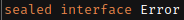
\includegraphics[width = 0.3\textwidth]{Imagenes/Fuentes/error_interface.png}
    \caption{Interfaz Error.}
    \label{fig:error_interface}
\end{figure}

En segundo lugar se ha creado la interfaz Result (se ha llamado así a pesar de que ya haya una clase con este nombre en la biblioteca estandar por considerarse el más apropiado). Esta es la interfaz principal que utilizan todas las funciones de la aplicación que devuelvan datos. Tiene dos parametros genéricos que cambiarán en cada caso específico -véase la figura \ref{fig:ejemplo_result}-, uno para los datos devueltos y otro para el tipo de error, también cuenta con los dos posibles resultados que pueda devolver una función que implemente esta interfaz: 
\begin{itemize}
    \item \textbf{Success}: para el caso de éxito. Llevará como parámetro los datos devueltos.
    \item \textbf{Error}: distinto de la interfaz explicada anteriormente, será lo que se devuelva en caso de error en la llamada a función y llevará como parámetro una clase que implemente la interfaz \textit{Error}.
\end{itemize}
\newpage
\begin{figure}[h]
    \centering
    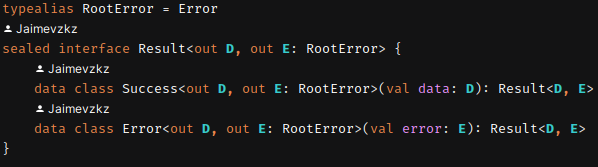
\includegraphics[width = 0.8\textwidth]{Imagenes/Fuentes/ejemplo_result.png}
    \caption{Interfaz Result.}
    \label{fig:ejemplo_result}
\end{figure}

\textbf{Result} y \textbf{Error} son las interfaces base del sistema. Lo siguiente será crear todas las interfaces que sean necesarias -e implementen \textit{Error}- para cada tipo de error. En Profinder solo ha sido necesario crear una que englobara todos los errores relativos a \hyperlink{subsec:firebase}{Firebase}, sin embargo, es un sistema escalable a futuro para múltiples tipos de errores.

Dentro de esta interfaz se declaran todos los tipos de errores (relativos a \hyperlink{subsec:firebase}{Firebase} por ejemplo, véase la figura \ref{fig:ejemplo_tipo_error}) como clases enumeradas, consiguiendo así que cada uno sea un enumerado que se gestiona de forma independiente en las distintas capas de la aplicación.
\begin{figure}[h]
    \centering
    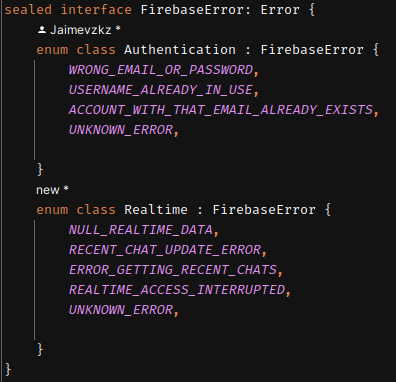
\includegraphics[width = 0.7\textwidth]{Imagenes/Fuentes/ejemplo_tipo_error.png}
    \caption{Ejemplo de tipo de error.}
    \label{fig:ejemplo_tipo_error}
\end{figure}

Con todo lo anterior, la gestión de errores se convierte en algo sencillo, las funciones deberán devolver un tipo \textit{Result} (figura \ref{fig:ejemplo_impl_result}).
\newpage
\begin{figure}[h]
    \centering
    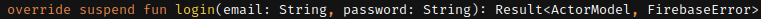
\includegraphics[width = 0.9\textwidth]{Imagenes/Fuentes/ejemplo_impl_result.png}
    \caption{Ejemplo de implementación de Result.}
    \label{fig:ejemplo_impl_result}
\end{figure}

Y en las llamadas a función se podrá gestionar si hay un error dividiendo los casos con una expresión
\textit{when}\hyperlink{cap:biblio}{\endnote{\textbf{when}: \url{https://www.programiz.com/kotlin-programming/when-expression}}}, como se ve en lafigura \ref{fig:llamada_funcion_result}.
\begin{figure}[h]
    \centering
    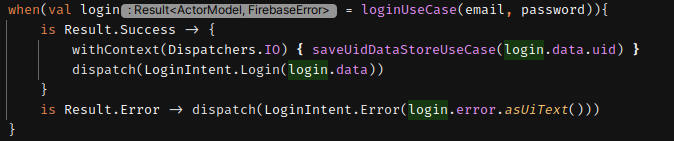
\includegraphics[width = 0.8\textwidth]{Imagenes/Fuentes/llamada_funcion_result.png}
    \caption{Ejemplo de llamada a función implementando Result.}
    \label{fig:llamada_funcion_result}
\end{figure}